\documentclass{article}
\usepackage[margin=0.75in]{geometry}
\usepackage{graphicx}
\graphicspath{ {./Images/} }

\title{A Brief Timeseries Analysis of VIX Closing Values}
\author{Varun Varanasi}

\begin{document}
\maketitle
\tableofcontents
\newpage

\section{Timeseries Plots}

\subsection{Daily Open}
\begin{center}
    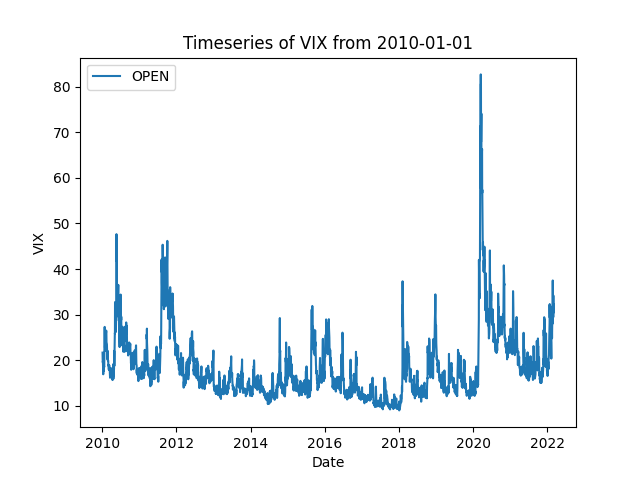
\includegraphics{VIX_Open_Timeseries_2010}
    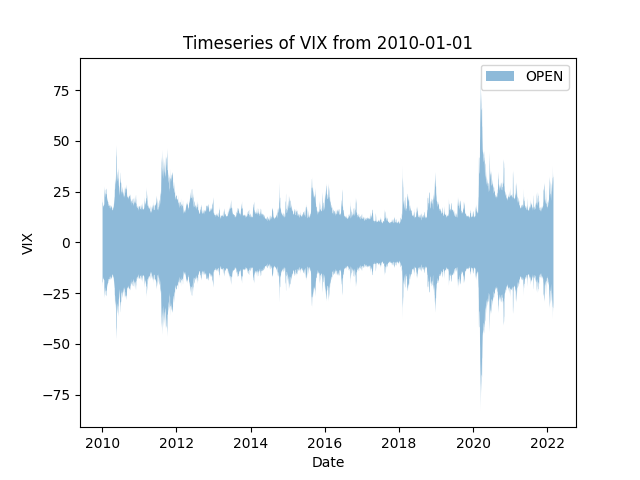
\includegraphics{VIX_Open_Timeseries_Fill_2010.png}
\end{center}

\subsection{Daily Close}
\begin{center}
    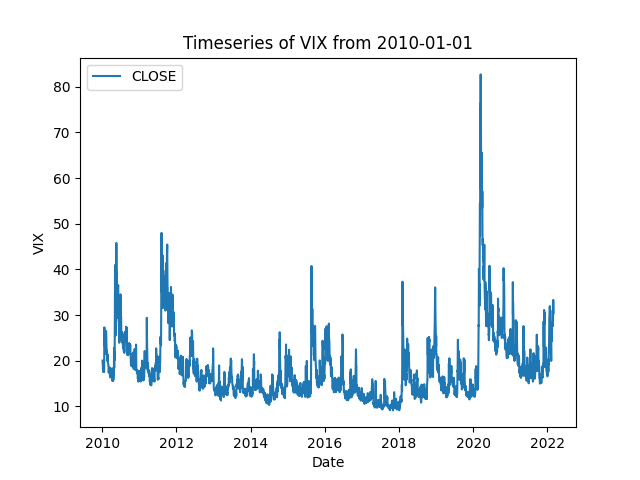
\includegraphics{VIX_Close_Timeseries_2010}
    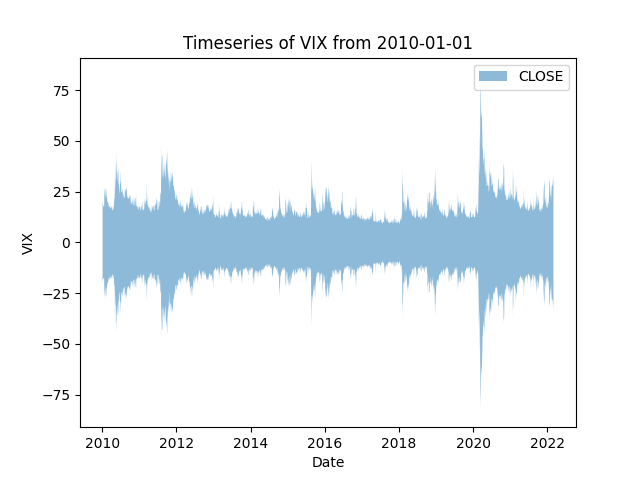
\includegraphics{VIX_Close_Timeseries_Fill_2010}
\end{center}

\subsection{Daily High}
\begin{center}
    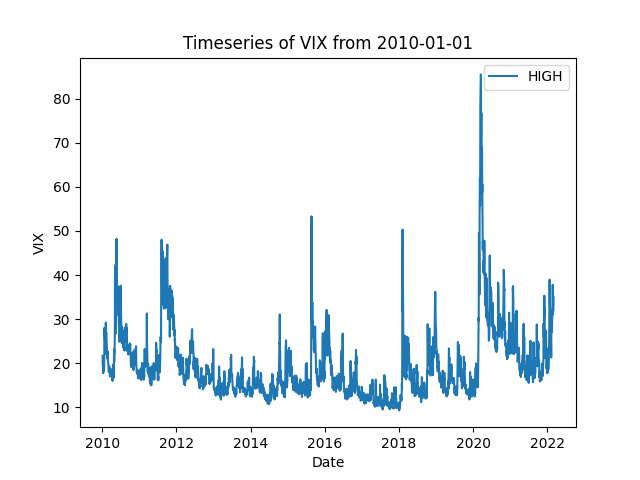
\includegraphics{VIX_High_Timeseries_2010}
    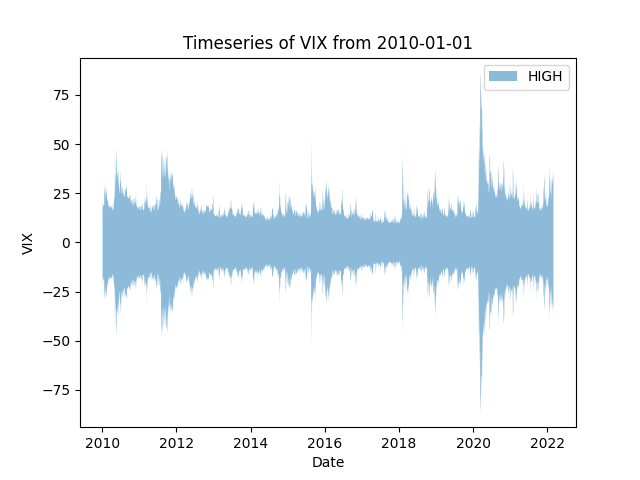
\includegraphics{VIX_High_Timeseries_Fill_2010}
\end{center}

\subsection{Daily Low}
\begin{center} 
    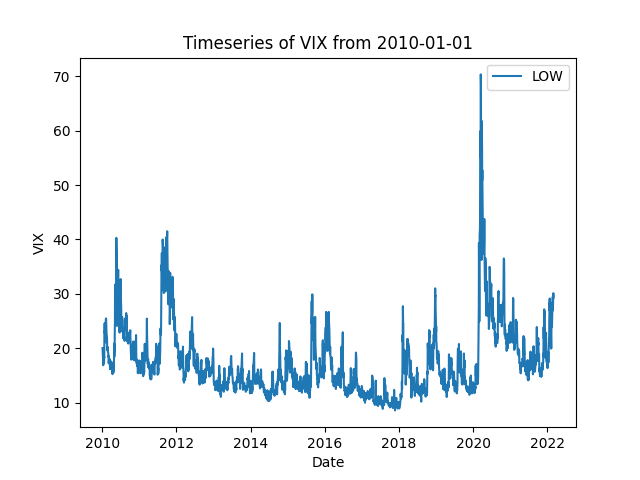
\includegraphics{VIX_Low_Timeseries_2010}
    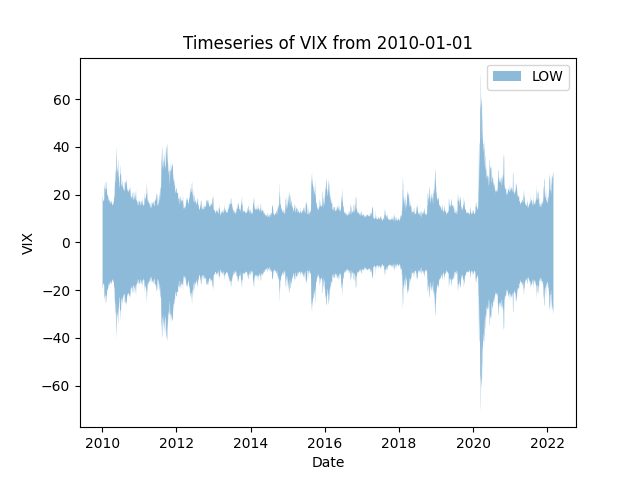
\includegraphics{VIX_Low_Timeseries_Fill_2010}
\end{center}

\section{Timeseries Decompositions}

\subsection{Multiplicative Decomposition}
A multiplicative time series uses the model: Value = Base Level x Trend x Seasonality x Error \\
Multiplicative models tend to be more common in economic datasets


\begin{figure}[h!]
    \centering
    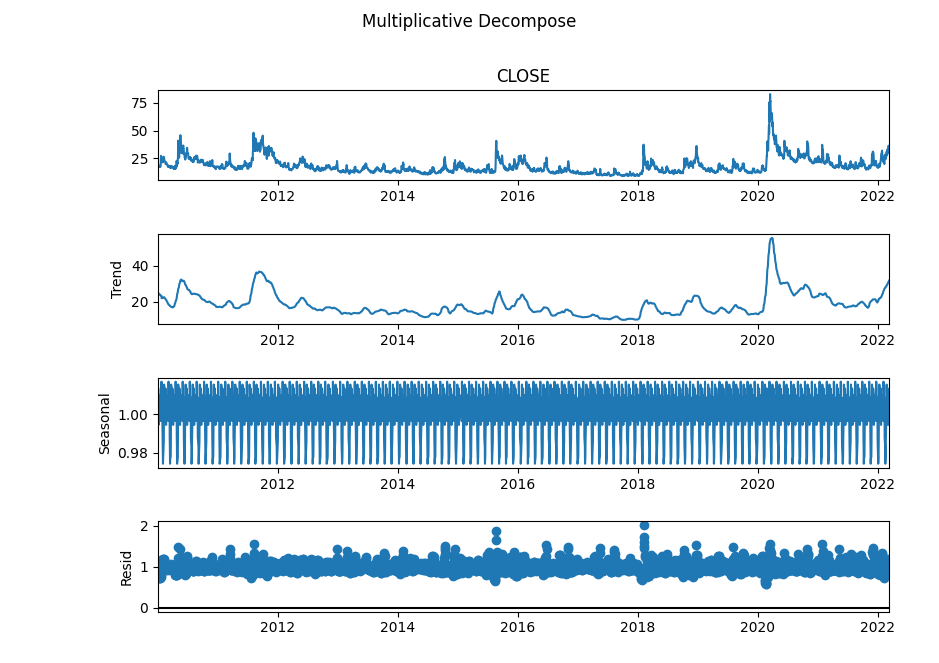
\includegraphics[width= 0.6\textwidth]{VIX_multiplicative_decomp_30_2010}
    \caption{Multiplicative Decomposition of VIX Closing Values with a period of 30 Days}
    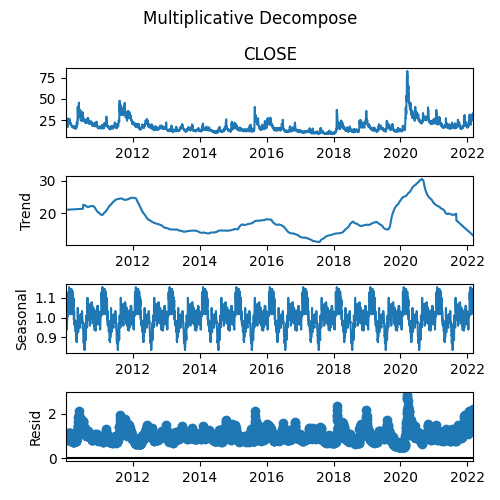
\includegraphics[width= 0.6\textwidth]{VIX_multiplicative_decomp_252_2010}
    \caption{Multiplicative Decomposition VIX Closing Values with a period of 252 Days}
\end{figure}

\newpage

\subsection{Additive Decomposition}
An additive time series model estimates the value by the equation Value = Base Level + Trend + Seasonality + Error

\begin{figure}[h!]
    \centering
    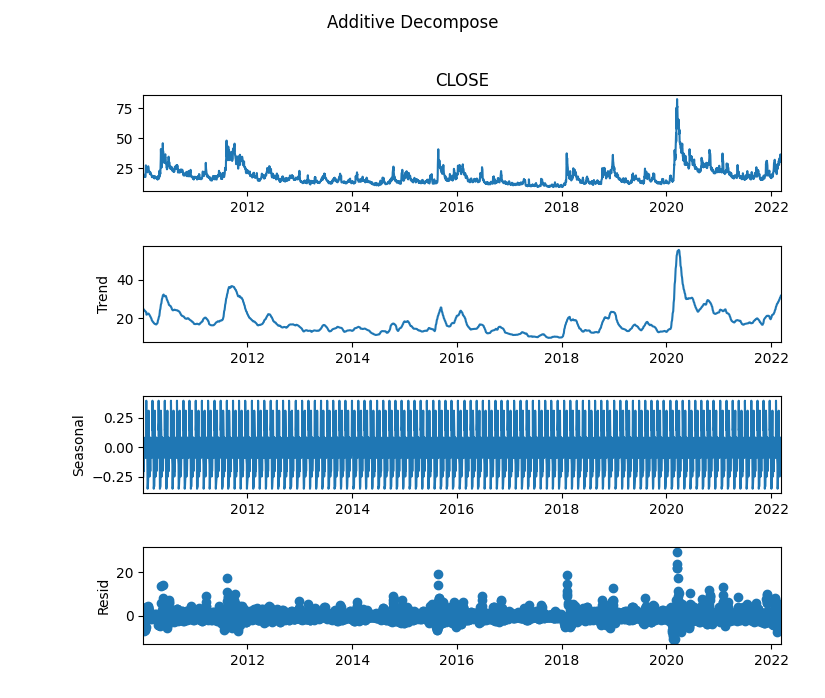
\includegraphics[width= 0.6\textwidth]{VIX_additive_decomp_30_2010}
    \caption{Additive Decomposition of VIX Closing Values with a period of 30 Days}
    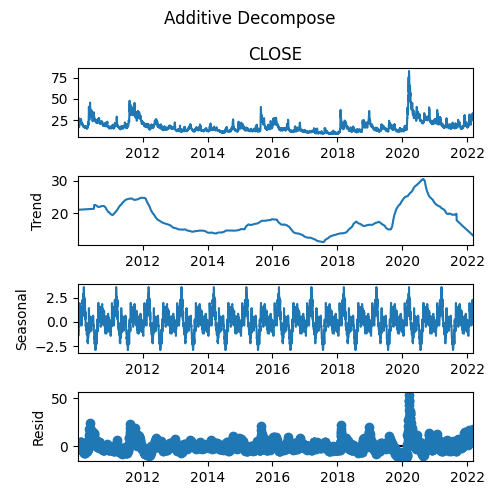
\includegraphics[width= 0.6\textwidth]{VIX_additive_decomp_252_2010}
    \caption{Additive Decomposition of VIX Closing Values with a period of 252 Days}
\end{figure}

\newpage

\section{Testing Stationarity}

A stationary time series is one that is independent of the time that it is observed. \\
Generally, predictions based on stationary series are more accurate than their non-stationary counter parts

\subsection{Augmented Dickey Fuller Test}
\begin{itemize}
    \item The null hypothesis of the ADH is that the series in question is non-stationary and posses a unit root
    \item We reject the null hypothesis for small p-values (less than 0.05)
    \item \textbf{VIX Closing Price ADH Test}: p-value = 9.9e-05
\end{itemize}


\section{Seasonality}

Autocorrelation plots reveal regular spikes in the data representative of seasonal timeseries variation \\
Unfortunately, in our VIX closing data there are no clear seasonality patterns in the autocorrelation plot
\begin{figure}[h!]
    \centering
    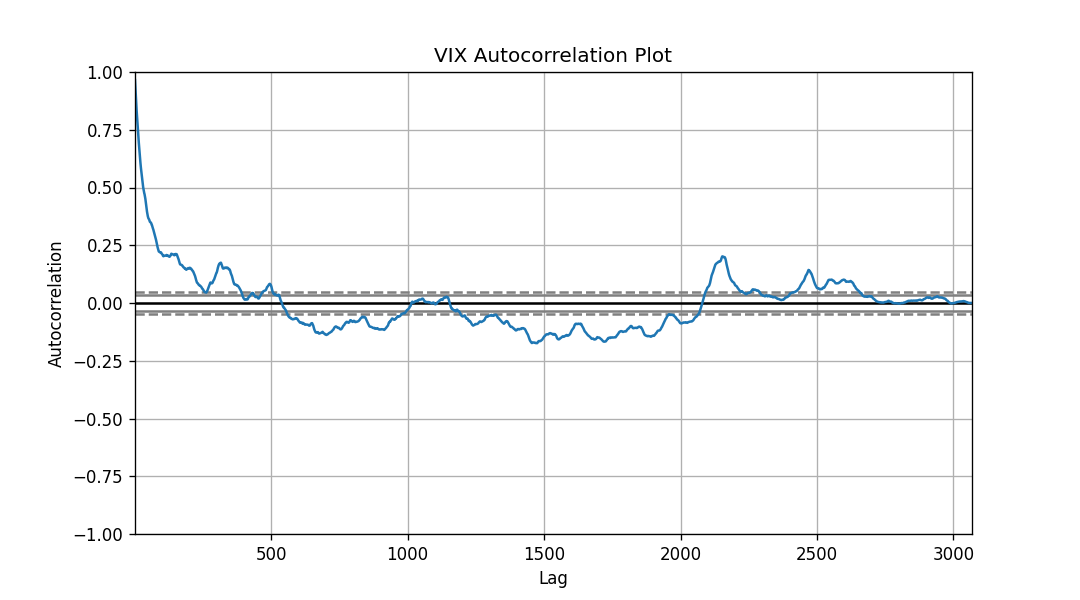
\includegraphics[width= 1\textwidth]{VIX_close_autocorrelation_2010.png}
    \caption{Autocorrelation of VIX closing values since 2010}
\end{figure}

\newpage

\section{Interpolating Missing Values}

\subsection{Linear Interpolation}
Linear interpolation a simple interpolation model where we estimated the more granular values via a line between the surrounding datapoints.

\begin{figure}[h!]
    \centering
    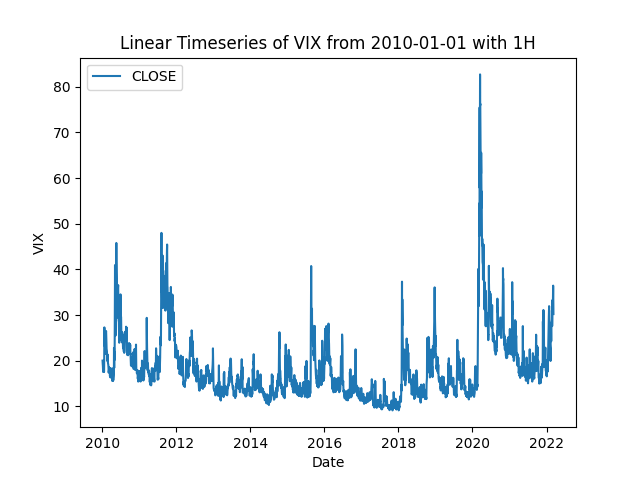
\includegraphics[width= 0.6\textwidth]{VIX_linear_interpolation_2010_1H.png}
    \caption{Timeseries of Linear Interpolation with 1 hour intervals}
\end{figure}

\subsection{Seasonal Interpolation}
In this interpolation method we first estimated the missing points via linear interpolation. To account for seasonal/random variation, we then modified each estimate by a noise factor drawn from a normal distribution centered at 0 with standard deviation equivalent to the sd. of the seasonal effects from a multiplicative decomposition. 

\begin{figure}[h!]
    \centering
    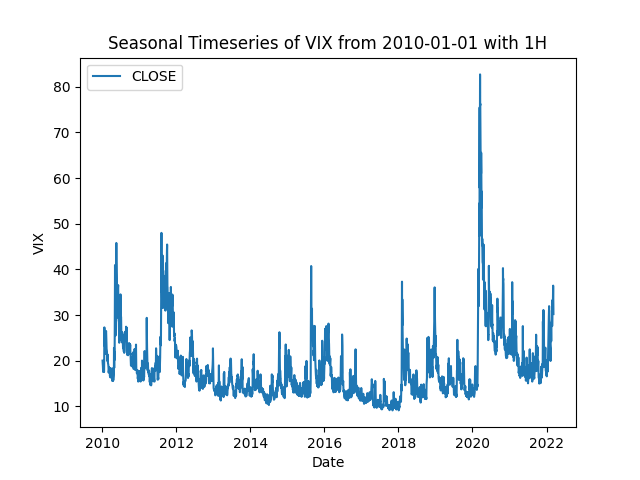
\includegraphics[width= 0.6\textwidth]{VIX_seasonal_interpolation_2010_1H.png}
    \caption{Timeseries of Seasonal Interpolation with 1 hour intervals}
\end{figure}


\newpage
\section{Granger Causality Test}
\begin{itemize}
    \item The Granger Causality test is a measure of how well one timeseries can predict another
    \item The test assumes that the times series in question (Y) is a function of its past values and another predictor timeseries (X)
\end{itemize}

\textbf{NEXT STEP: APPLY GRANGER CAUSALITY TEST TO VIX AND METACULUS DATA}

\end{document}